%--------------------------------------------
%%%%%%%%%%%%%%%%%%%%%%%%%%%%%%%%%%%%%%%%%%%%%%%%%%%%
% THE PREAMBLE
%%%%%%%%%%%%%%%%%%%%%%%%%%%%%%%%%%%%%%%%%%%%%%%%%%%%
%--------------------------------------------

%%%%%%%%%%%%%%%%%%%%%%%%%%%%%%%%%%%%%%%%%%%%%%%%%%%%
% DOCUMENT CLASS (don't ever change this unless specified to do so).
%%%%%%%%%%%%%%%%%%%%%%%%%%%%%%%%%%%%%%%%%%%%%%%%%%%% 
\documentclass[11pt]{article}


%%%%%%%%%%%%%%%%%%%%%%%%%%%%%%%%%%%%%%%%%%%%%%%%%%%%
% USEFUL PACKAGES THAT YOU NEED. (Everything here needs to be here for the program to run.  Do not delete anything from the preamble, but you can add new things that you find on the internet.)
%%%%%%%%%%%%%%%%%%%%%%%%%%%%%%%%%%%%%%%%%%%%%%%%%%%%
\usepackage{fullpage}
\usepackage{amsfonts}
\usepackage{amsmath}
\usepackage{amsthm}
\usepackage{graphicx}
\usepackage{color}
\usepackage{amssymb}
\usepackage{empheq}
\usepackage{mathrsfs}
\usepackage{enumerate}
\usepackage{tikz}
\usepackage{pgflibraryarrows}
\usepackage{pgflibrarysnakes}
\usepackage{upgreek}
\usepackage{tipa}
\usepackage{gensymb}
\usepackage{multicol}
\usepackage{textcomp}


%%%%%%%%%%%%%%%%%%%%%%%%%%%%%%%%%%%%%%%%%%%%%%%%%%%%
% CREATES A SOLUTION ENVIRONMENT FOR HOMEWORK ASSIGNMENTS (You may not use this but leave it here for future assignments)
%%%%%%%%%%%%%%%%%%%%%%%%%%%%%%%%%%%%%%%%%%%%%%%%%%%%
\usepackage{versions}
\excludeversion{sol}
\includeversion{sol}
\newenvironment{solution}{
\sol\\{\sc{Solution:}}}{
$\hfill\blacksquare$\endsol}


%%%%%%%%%%%%%%%%%%%%%%%%%%%%%%%%%%%%%%%%%%%%%%%%%%%%
% CUSTOM DEFINITIONS FOR CREATING DERIVATIVE SYMBOLS (You will definitely use these.)
%%%%%%%%%%%%%%%%%%%%%%%%%%%%%%%%%%%%%%%%%%%%%%%%%%%%
\newcommand{\pd}[2]{\frac{\partial #1}{\partial #2}}
\newcommand{\pdd}[2]{\frac{\partial^2 #1}{\partial {#2}^2}}
\newcommand{\de}[2]{\frac{d #1}{d #2}}
\newcommand{\dde}[2]{\frac{d^2 #1}{d #2^2}}

%%%%%%%%%%%%%%%%%%%%%%%%%%%%%%%%%%%%%%%%%%%%%%%%%%%%
% CREATES THE TITLE PAGE (Note where to put the author, title, and date.)
%%%%%%%%%%%%%%%%%%%%%%%%%%%%%%%%%%%%%%%%%%%%%%%%%%%%
\title{\textsc{Mariam Avagyan}}
\author{\Large{MATH 210 -- 01 -- \textsc{Scientific Computing in Matlab}}}
\date{December 24, 2015}


%%%%%%%%%%%%%%%%%%%%%%%%%%%%%%%%%%%%%%%%%%%%%%%%%%%%
% CREATES A HEADER FOR EACH PAGE.  Please note where the left, center, and right titles are:
%%%%%%%%%%%%%%%%%%%%%%%%%%%%%%%%%%%%%%%%%%%%%%%%%%%%
\usepackage{fancyhdr}
\setlength{\headheight}{15.2pt}
\pagestyle{fancy}
\setlength\headsep{30pt}
\lhead{Mariam Avagyan}   					%  Your name on the left header.
\chead{\textsc{MATLAB Final Project}}			%  Title in the center.
\rhead{\today}							%  Date on the right header.

\begin{document}

\maketitle
\pagebreak

%--------------------------------------------
%%%%%%%%%%%%%%%%%%%%%%%%%%%%%%%%%%%%%%%%%%%%%%%%%%%%
% END OF THE PREAMBLE AND BEGINNING OF THE ACTUAL DOCUMENT
%%%%%%%%%%%%%%%%%%%%%%%%%%%%%%%%%%%%%%%%%%%%%%%%%%%%
%--------------------------------------------


%%%%%%%%%%%%%%%%%%%%%%%%%%%%%%%%%%%%%%%%%%%%%%%%%%%%
% SECTIONS, SUBSECTIONS, EQUATIONS, and OTHER THINGS:
%%%%%%%%%%%%%%%%%%%%%%%%%%%%%%%%%%%%%%%%%%%%%%%%%%%%

\section{Setup}

A Julia set is a complementary set that consists of iterations of a function. The values of this function play a crucial role in generating a Julia set. Any small deviation can cause drastic changes in the sequence. This is why the behavior of a Julia set is called 'chaotic'. By simply changing the real and imaginary parts of a complex number, one can easily plot various graphs of any Julia set (this property will be discussed more in depth in the "Methods" section).
The Julia set is named after the French mathematicians Gaston Julia. He studied complex dynamics during the early 20th century.

Given two complex numbers, $c$ and $Z$, let's define the following recursive function:
   
\begin{center}
$Z_{n+1} = {Z_n}^2+c$
\end{center}

This function is a dynamical system called a quadratic map. Depending on the values of $c$ and $Z_0$, the sequence of numbers $Z_1$, $Z_2$, $Z_3$,... (so-called "orbit" of $Z_0$) tends towards infinity, goes into a periodic loop or dances around the complex plane (this is an example of "chaos"). These starting values, c and $Z_0$, make up the Julia set of the map, denoted $J_c$.
In this problem, we will write a MATLAB script that visualizes 7 different Julia sets.

\section{Methods}

The most efficient way to solve this problem is to write a function that will accept various inputs and will plot the corresponding maps. It can be seen in the m-file and .html-file that a function $function [Z,W] = Avagyan-Final-Function(iter,N,zMax,a,b)$ was written. To plot different Julia sets, one would need to input different values for the inputs $iter$, $N$, $zMax$, $a$, and $b$ to obtain graphs. However, it is hard to find inputs that will results in beautiful graphs. That's why the entire function was turned into a comment. Instead, specific values of inputs were tested and plotted. The maps will be seen in the "Visual Interpretation" section.

The functions $pcolor$ and $imagesc$ were used to obtain a map. Both of these functions give a view from the top. The function $colormap$ was used to color the fractal map. To iterate the function, a $for$ loop was used. After trial and error, it was decided to plot the variable $W = e^{-|Z|}$ since $pcolor$ and $imagesc$ could have only real input values. The reason why an exponential graph was chosed is because it resulted in more beautiful graphs and worked for all the sets.
The function $shading$ with option $flat$ was used to make the graphs more pleasant for the eye.


\section{Visual Interpretation}
The following maps represent different complex numbers.
\begin{center}
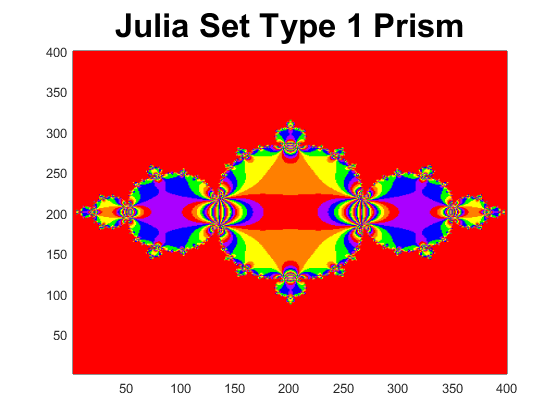
\includegraphics[width=\textwidth] {Set_1_prism.png}
\end{center}



\section{Conclusion}

This project not only sparkled my interest in Math but also helped me learn more commands in MATLAB. I played with mapping for about two days.

Since the functions $pcolor$ and $imagesc$ both need real input variables the command $pcolor(Z)$ gave errors. It took me a while to realize that instead a new real variable $W$ depending on $Z$ could be plotted. I got the idea of defining $W$ to be an exponential function from Wikipedia because they showed many examples of Julia sets with exponential functions.

Since Julia sets are infinitely thin, I tried to zoom in my plots which turned out to be a disaster. The image resolution was terrible. I tried to find a way to plot maps with better resolution. However, I did not find an easy way to do so. My future goal is to solve this problem.

%%%%%%%%%%%%%%%%%%%%%%%%%%%%%%%%%%%%%%%%%%%%%%%%%%%%
% DOCUMENT END
%%%%%%%%%%%%%%%%%%%%%%%%%%%%%%%%%%%%%%%%%%%%%%%%%%%%
\end{document}